\chapter{Machine Learning, Tecniche e Concetti}
\label{ch:capitolo2}
Questo capitolo si propone di esplorare i concetti teorici fondamentali del ML nel contesto dell'applicazione medica, con particolare attenzione alla riabilitazione dei pazienti con malattie cardiache.
% --- Inizio del Capitolo 2 ---

\section{Machine Learning, un Introduzione}
\begin{flushleft}
    

"Il Machine Learning (ML) è la branca dell'informatica che dà ai computer la capacità di apprendere senza essere  senza esser stati esplicitamente programmati."\cite{HandsOnML}
Il processo di apprendimento in ML si basa su diversi concetti fondamentali, ma tutto parte dai dati.
Essi possono essere di diversi tipi, come dati strutturati (ad esempio tabelle CSV) o non strutturati (come immagini o testo). L'obiettivo principale è quello di estrarre conoscenza e informazioni dai dati al fine di prendere decisioni o effettuare previsioni.

I dati utilizzati nel processo di apprendimento sono spesso chiamati istanze e sono caratterizzati da un insieme di features che rappresentano le loro proprietà e caratteristiche. Quando si lavora con un numero 
$n$ di features, i dati possono essere rappresentati come punti o vettori in uno spazio
$n$-dimensionale (figura \ref{fig:puntispazion}).

\begin{figure}[H]
    \centering
    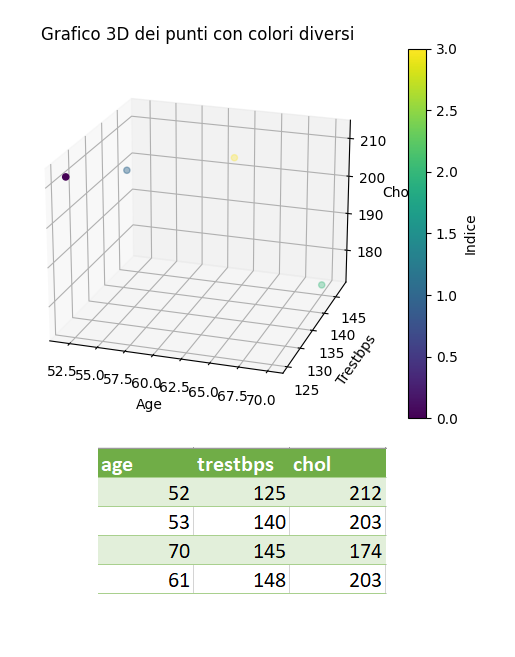
\includegraphics[scale=0.8]{TemplateTesi/immagini/tabellaplot3dbb.png}
    \caption{Da dati tabellari a Visualizzazione nello spazio}
    \label{fig:puntispazion}
\end{figure}



A seconda dell'obiettivo dell'apprendimento e della tipologia dei dati disponibili, possiamo distinguere tra:
metodi di \textbf{apprendimento supervisionato} e metodi di \textbf{apprendimento non supervisionato}. 
Nel caso dell'apprendimento supervisionato, i dati osservati sono associati a etichette, che possono essere valori categorici o numerici, rappresentando ciò che deve essere appreso in modo automatico. In pratica, si dispone di esempi in cui è nota l'etichetta corretta, e si cerca di costruire un modello che possa predire le etichette per nuovi dati in ingresso. 

I metodi di apprendimento non supervisionato, invece, mirano a estrarre informazioni di vario tipo da un insieme di osservazioni non etichettate. Questi metodi possono essere utilizzati, ad esempio, per raggruppare i dati in base alle loro somiglianze.

\subsection{Tipologie di Problemi Affrontabili}
Il ML può essere applicato a una vasta gamma di problemi. Le tipologie principali di problemi affrontabili includono:

\subsubsection{Classificazione}
La classificazione è un problema di apprendimento supervisionato in cui l'obiettivo è assegnare un'etichetta o una categoria a un'istanza di dati sulla base delle sue caratteristiche.
La classificazione  si dice \emph{binaria} se le classi di output sono esattamente due, come 0 e 1, \emph{multiclasse} altrimenti.
Ad esempio, in medicina, può essere utilizzato per classificare i tumori come benigni o maligni in base alle loro caratteristiche diagnostiche.

\begin{figure}[H]
    \centering
    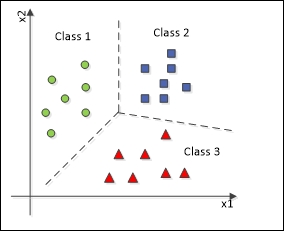
\includegraphics[scale=0.8]{TemplateTesi/immagini/B04971_06_01.jpg}
    \caption{Esempio di Classificazione multiclasse \cite{ImmClassificazione}}
    \label{fig:my_label}
\end{figure}

\subsubsection{Regressione}

La regressione si occupa di stimare o predire un valore numerico continuo sulla base delle variabili in input. 
L’obiettivo della regressione diventa dunque quello di realizzare un modello matematico che sia in grado di rappresentare una correlazione tra le features disponibili dell’input e quello che invece è il valore atteso. Questo tipo di problema è comunemente utilizzato in ambito clinico per determinare la relazione tra  diversi fattori e gli esiti delle malattie, o per identificare fattori prognostici rilevanti.\cite{Regressione}
Anche in questo caso è una tipologia di problema che risiede tra quelli di apprendimento supervisionato.
\begin{figure}[H]
    \centering
    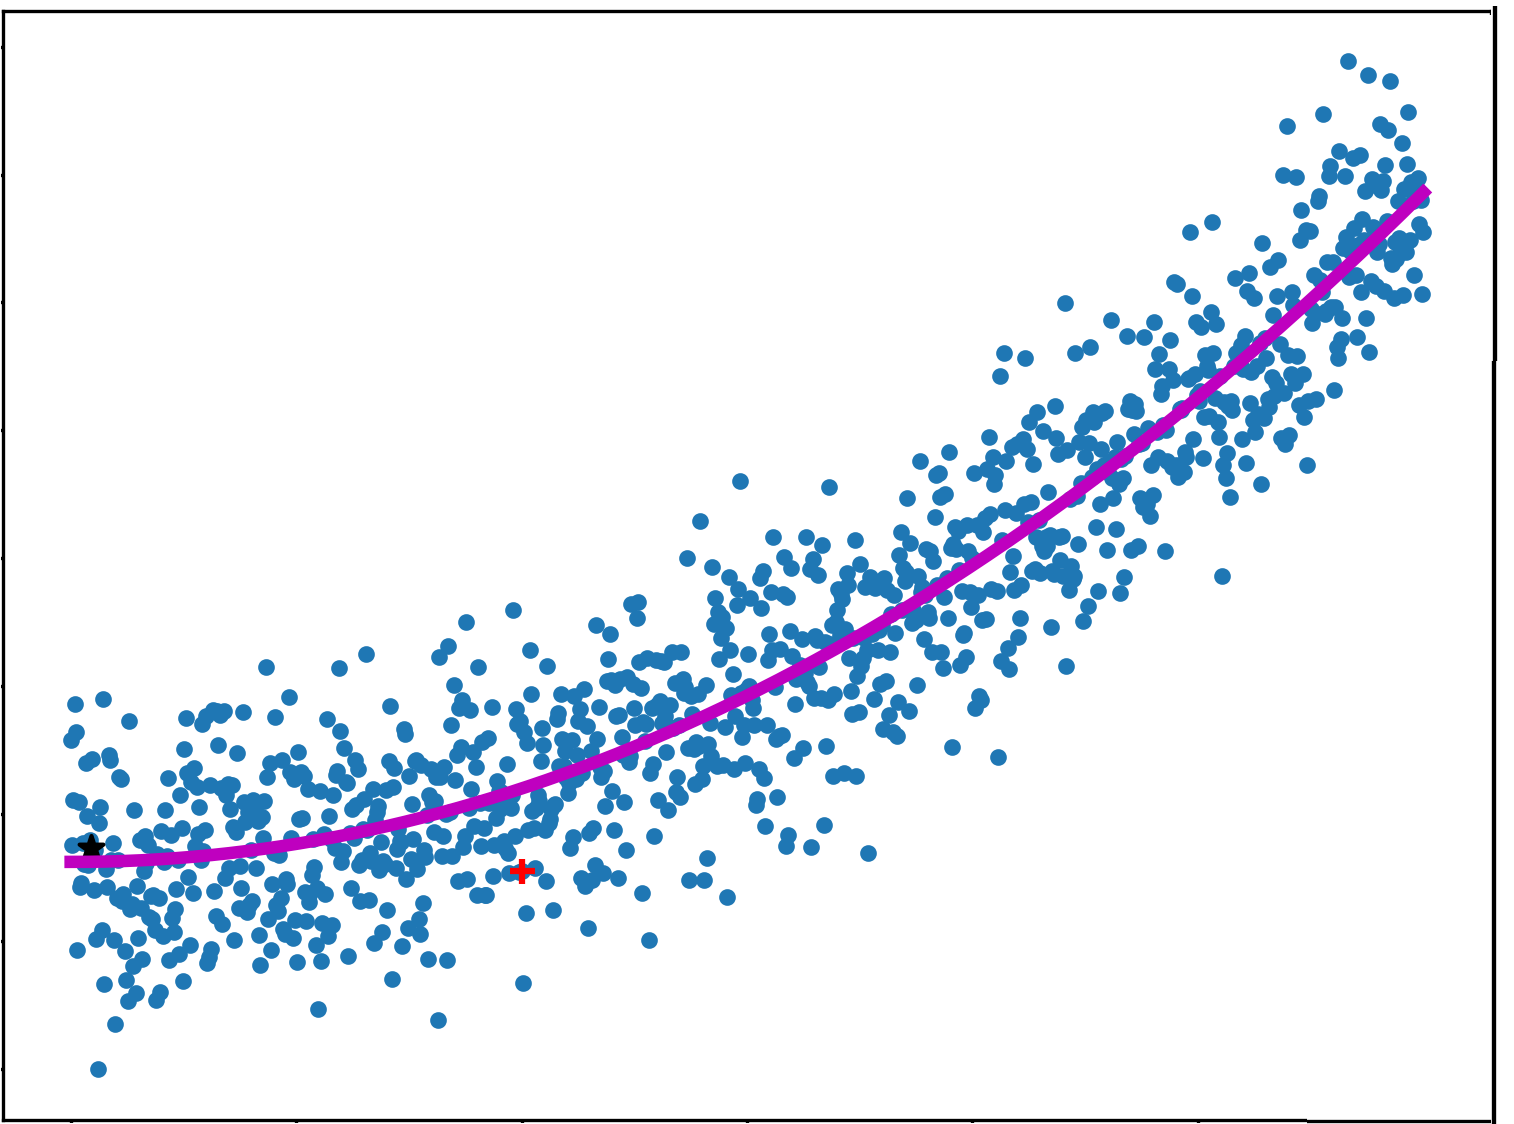
\includegraphics[scale=0.15]{TemplateTesi/immagini/TCH45-06 (1).png}
    \caption{Esempio di Regressione \cite{ImmRegressione}}
    \label{fig:my_label}
\end{figure}

\subsubsection{Clustering}

Il clustering consiste nel raggruppare gli oggetti in base alle loro somiglianze. Questo approccio può essere utilizzato per identificare sottogruppi di pazienti con caratteristiche comuni.
A differenza delle problematiche sopra descritte il clustering si basa su un apprendimento \emph{non} supervisionato.


\begin{figure}[H]
    \centering
    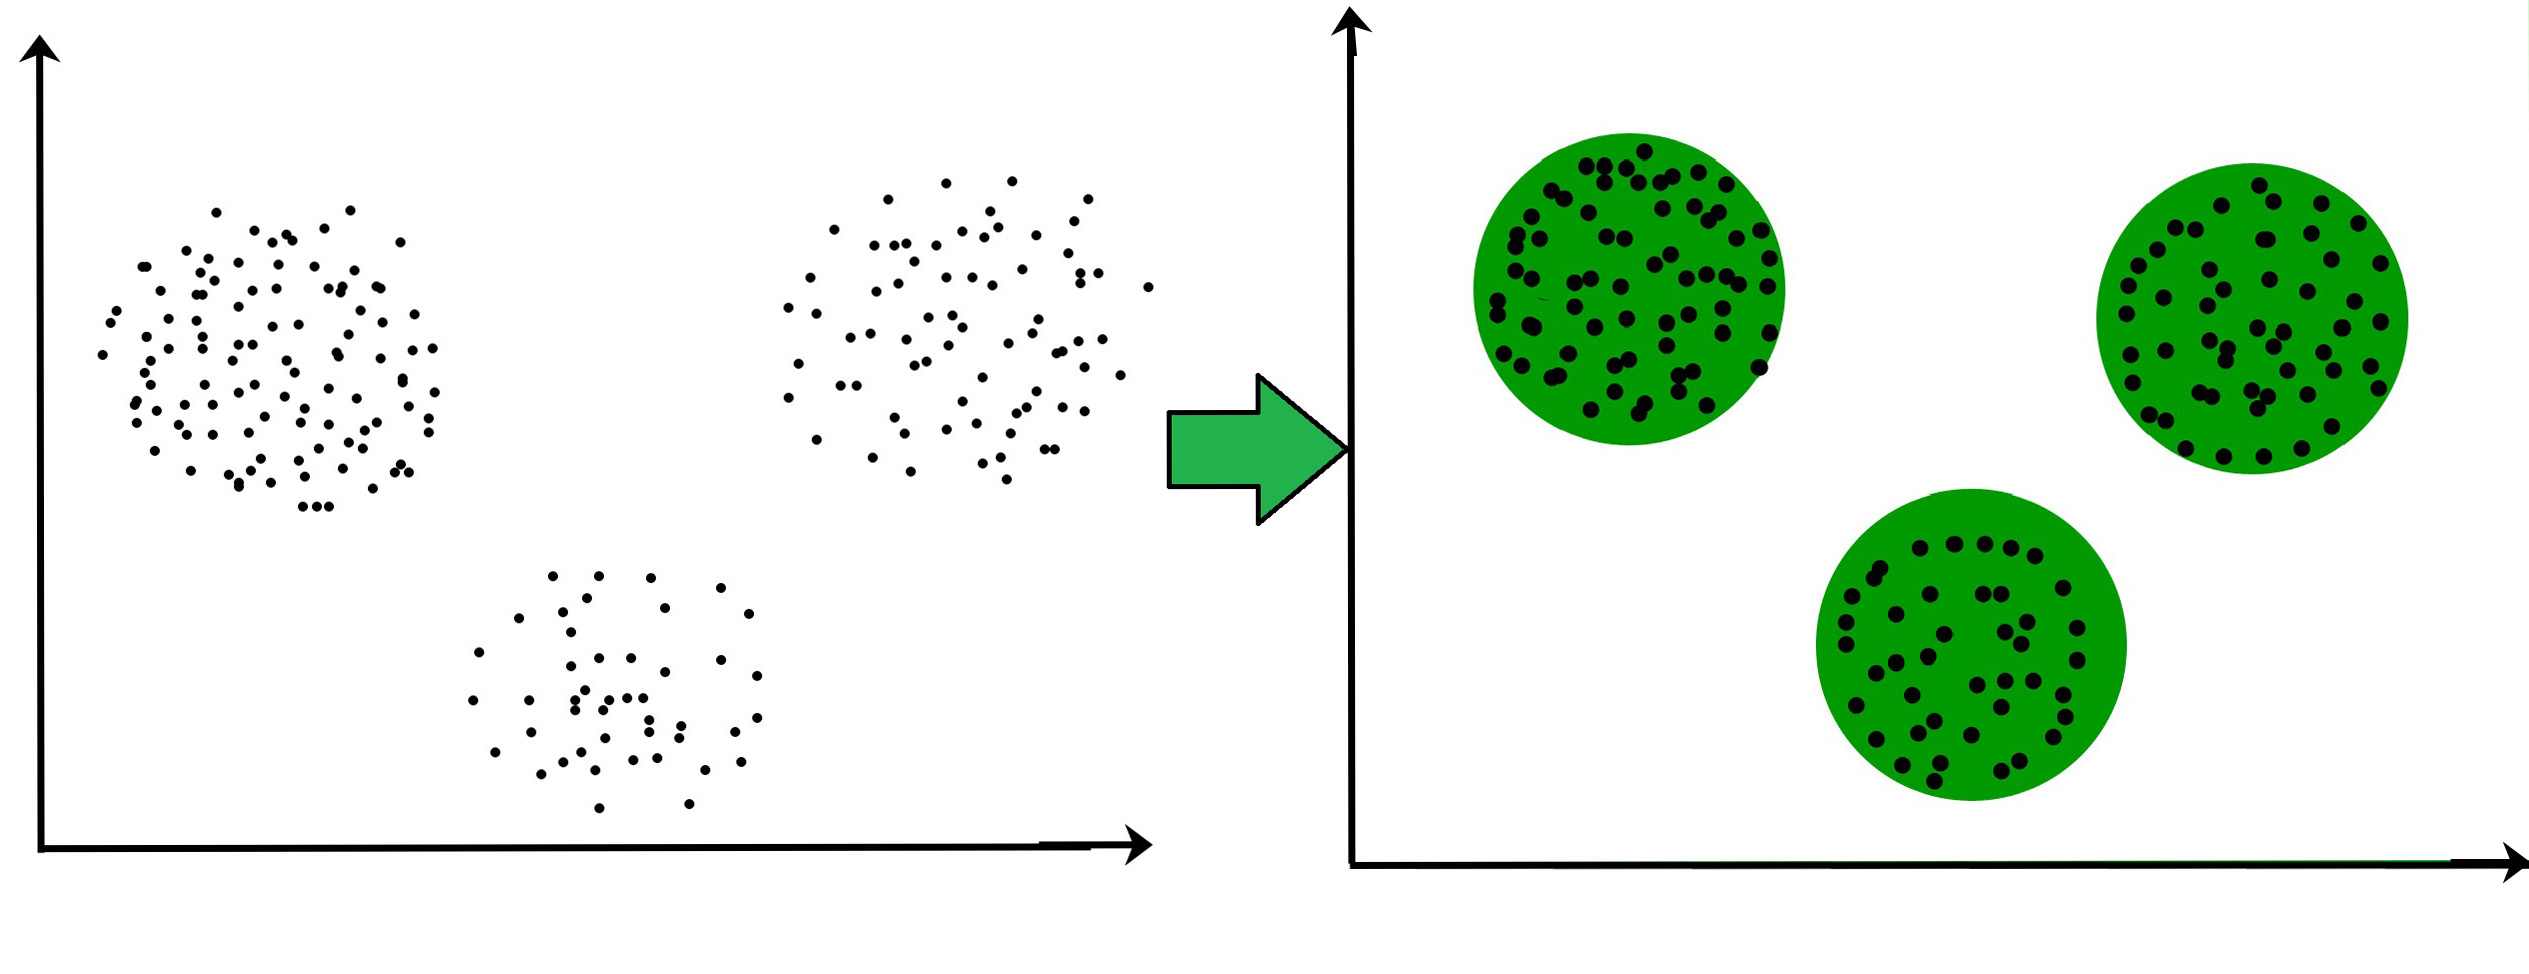
\includegraphics[scale=0.4]{TemplateTesi/immagini/merge3cluster.jpg}
    \caption{Esempio di Clustering \cite{ImmClustering}}
    \label{fig:my_label}
\end{figure}

\begin{figure}[H]
    \centering
    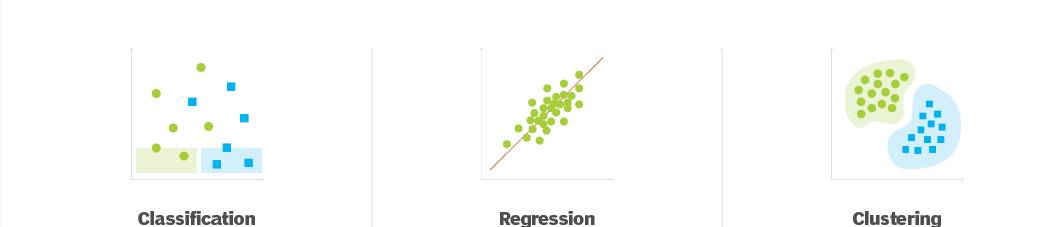
\includegraphics[scale=0.6]{TemplateTesi/immagini/businessanalytics-leading_data_science_techniques-fcut.png}
    \caption{Tipologie principali di problemi in ML \cite{ImmProblemiML}}
    \label{fig:my_label}
\end{figure}
\end{flushleft}

\section{Problematiche tipiche nel Machine Learning}
Il ML non è esente da problematiche. In questa sezione, esamineremo le principali sfide associate all'uso del ML, quali sbilanciamento delle classi, gli outlier, il continuo adattamento del modello e il bias nei dati.

\subsection{Sbilanciamento}
\begin{flushleft}
    
Nella maggior parte dei casi reali, i dataset utilizzati per addestrare i modelli di ML possono essere sbilanciati. Ciò significa che una classe di interesse può essere rappresentata da un numero significativamente inferiore di esempi rispetto ad altre classi. Lo sbilanciamento dei dati può portare a problemi nella fase di addestramento, poiché i modelli tendono ad essere influenzati dalle classi più numerose, ignorando le classi minoritarie, portando a previsioni inaccurate e a scarsa generalizzazione.

Per risolvere questa problematica possiamo attuare due approcci principali: \emph{oversampling} della classe minoritaria e \emph{undersampling} della classe maggioritaria. 

\subsubsection{Oversampling}
\begin{figure}[H]
    \centering
    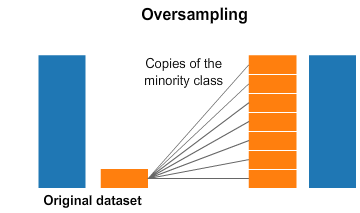
\includegraphics[scale=0.6]{TemplateTesi/immagini/oversamp.png}
    \caption{Oversampling in Dataset sbilanciato \cite{ImmOverUnderSampling}}
    \label{fig:my_label}
\end{figure}
L'oversampling è una tecnica di bilanciamento del dataset in cui le istanze della classe minoritaria vengono duplicate o generate sinteticamente per aumentare la loro frequenza nel dataset di addestramento.
Un algoritmo che implementa tale tecnica è lo \emph{SMOTE} (Synthetic Minority Oversampling Technique), questo genera nuovi campioni sintetici della classe minoritaria attraverso l'interpolazione tra i campioni di minoranza esistenti.
Il processo di interpolazione viene effettuato creando nuovi campioni sintetici lungo le linee che collegano i campioni di minoranza vicini (figura \ref{fig:smote}).


\begin{figure}[H]
    \centering
    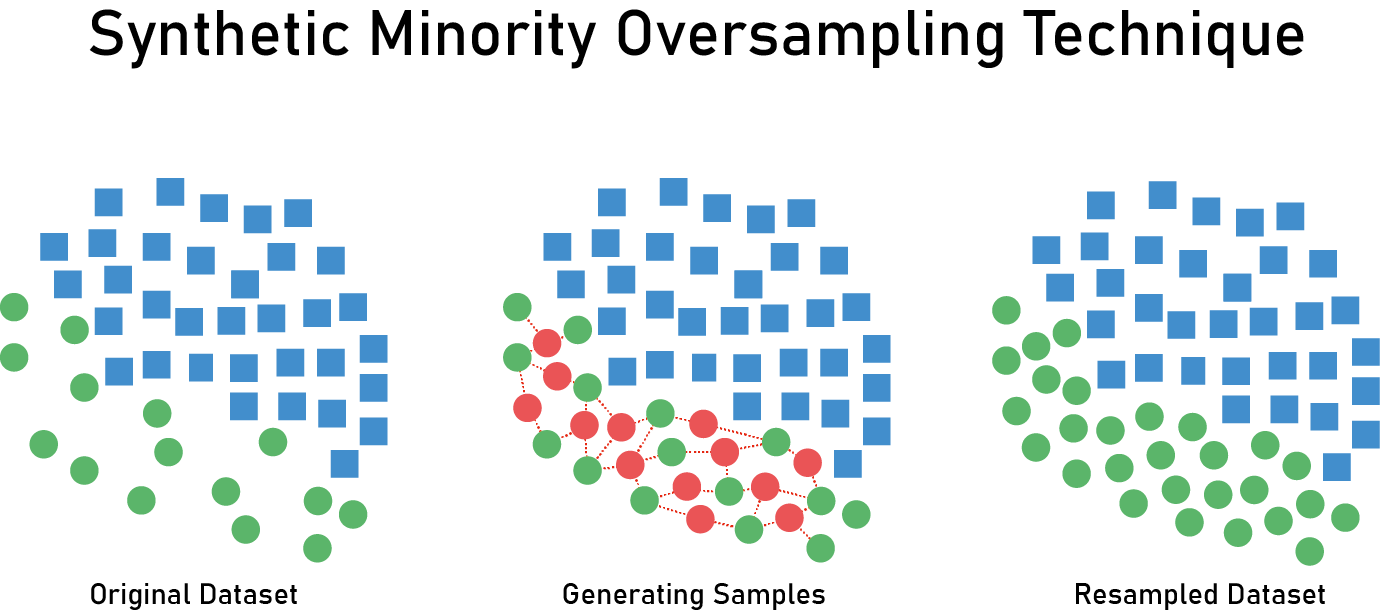
\includegraphics[scale=0.2]{TemplateTesi/immagini/smote.png}
    \caption{Funzionamento dello SMOTE}
    \label{fig:smote}
\end{figure}

\subsubsection{Undersampling}

\begin{figure}[H]
    \centering
    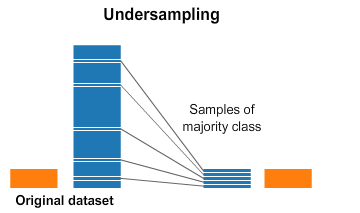
\includegraphics[scale=0.6]{TemplateTesi/immagini/undersamp.png}
    \caption{Undersampling in Dataset sbilanciato  \cite{ImmOverUnderSampling}}
    \label{fig:my_label}
\end{figure}
L'undersampling è una tecnica di bilanciamento del dataset in cui le istanze della classe maggioritaria vengono rimosse per ridurre la loro frequenza nel dataset di addestramento.
Gli algoritmi che ho valutato per la gestione dell'undersampling sono il \emph{Tomek Link} e l'\emph{ENN (Edited Nearest Neighbour)}.
Il Tomek Link (figura \ref{fig:tomek}) identifica le coppie di istanze che appartengono a classi diverse che sono molto vicine tra loro, rimuovendo il record della classe maggioritaria dal dataset di training.
L'ENN invece seleziona un insieme di K punti della classe minoritaria e l'insieme dei punti della classe maggioritaria più vicini ad essi\ref{fig:enn}),rimuovendo i suddetti punti della classe maggioritaria.
In entrambi i casi riduciamo la sovrapposizione tra le classi aumentando la distanza tra le istanze, migliorando la capacità del modello di distinguere tra le classi.
È bene tenere di conto però che parametri di selezione troppo stringenti possono portare ad una perdita di informazione e conseguentemente una precisione minore da parte del modello.

\begin{figure}[H]
    \centering
    
\includegraphics[scale=0.4]{TemplateTesi/immagini/tomek.png}
    \caption{Funzionamento del Tomek Link \cite{ImmTOmekLink}}
    \label{fig:tomek}
\end{figure}


\begin{figure}[H]   
    \centering
    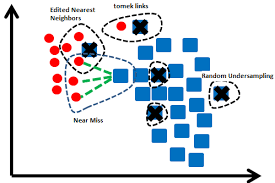
\includegraphics[scale=0.7]{TemplateTesi/immagini/enn.png}
    \caption{Funzionamento dell'ENN \cite{ImmENN}}
    \label{fig:enn}
\end{figure}


\subsection{Outliers}
Gli outliers sono dati che si discostano significativamente dagli altri punti della stessa distribuzione o cluster, i problemi legati ad essi sono l’identificazione e la cancellazione degli stessi

\subsubsection{Z-Score}

\begin{figure}[H]
    \centering
    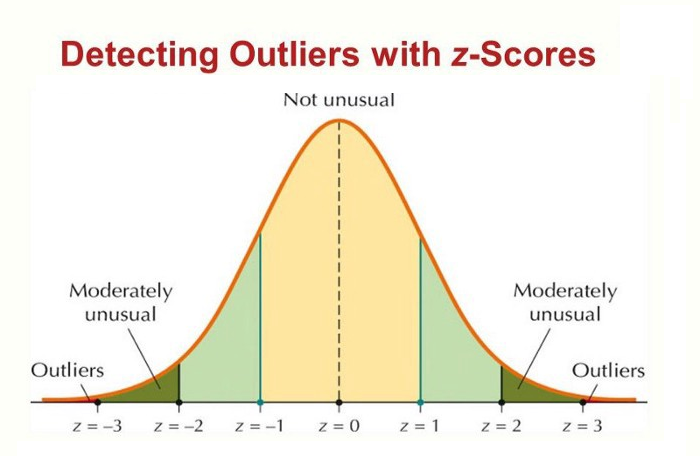
\includegraphics[scale=0.3]{TemplateTesi/immagini/Zscore.png}
    \caption{Zscore per rilevazione e cancellazione degli outlier \cite{ImmZscore}}
    \label{fig:zscore}
\end{figure}

Lo Z-score è una tecnica utilizzata per rilevare e cancellare gli outlier nei dataset, utilizza la deviazione standard e la media dei dati per identificare i valori che si discostano significativamente dalla media.
Il suo funzionamento segue la formula:

$$Z=\frac{X- \mu}{\sigma}$$
                                      
dove:
\begin{itemize}
    \item $\mu=deviazione  standard$
    \item $\sigma=media$
\end{itemize}



Una volta che avremo deciso un valore soglia "$n$" verranno eliminati tutti i punti distanti $n$ deviazioni standard dalla media.


\subsubsection{IQR Score}
L'IQR, Interquartile Range, è una misura della dispersione utilizzata per rilevare gli outlier nei dataset.
Ci basiamo sulla suddivisione in quartili della distribuzione dei dati per cancellare i valori che si discostano troppo dalla mediana.
L'outlier viene identificato come tale quando il suo valore è al di fuori di un intervallo soglia specificato.
Valori soglia standard sono di solito 1,5 oppure 3 volte la deviazione interquartile.
\begin{figure}[H]
    \centering
    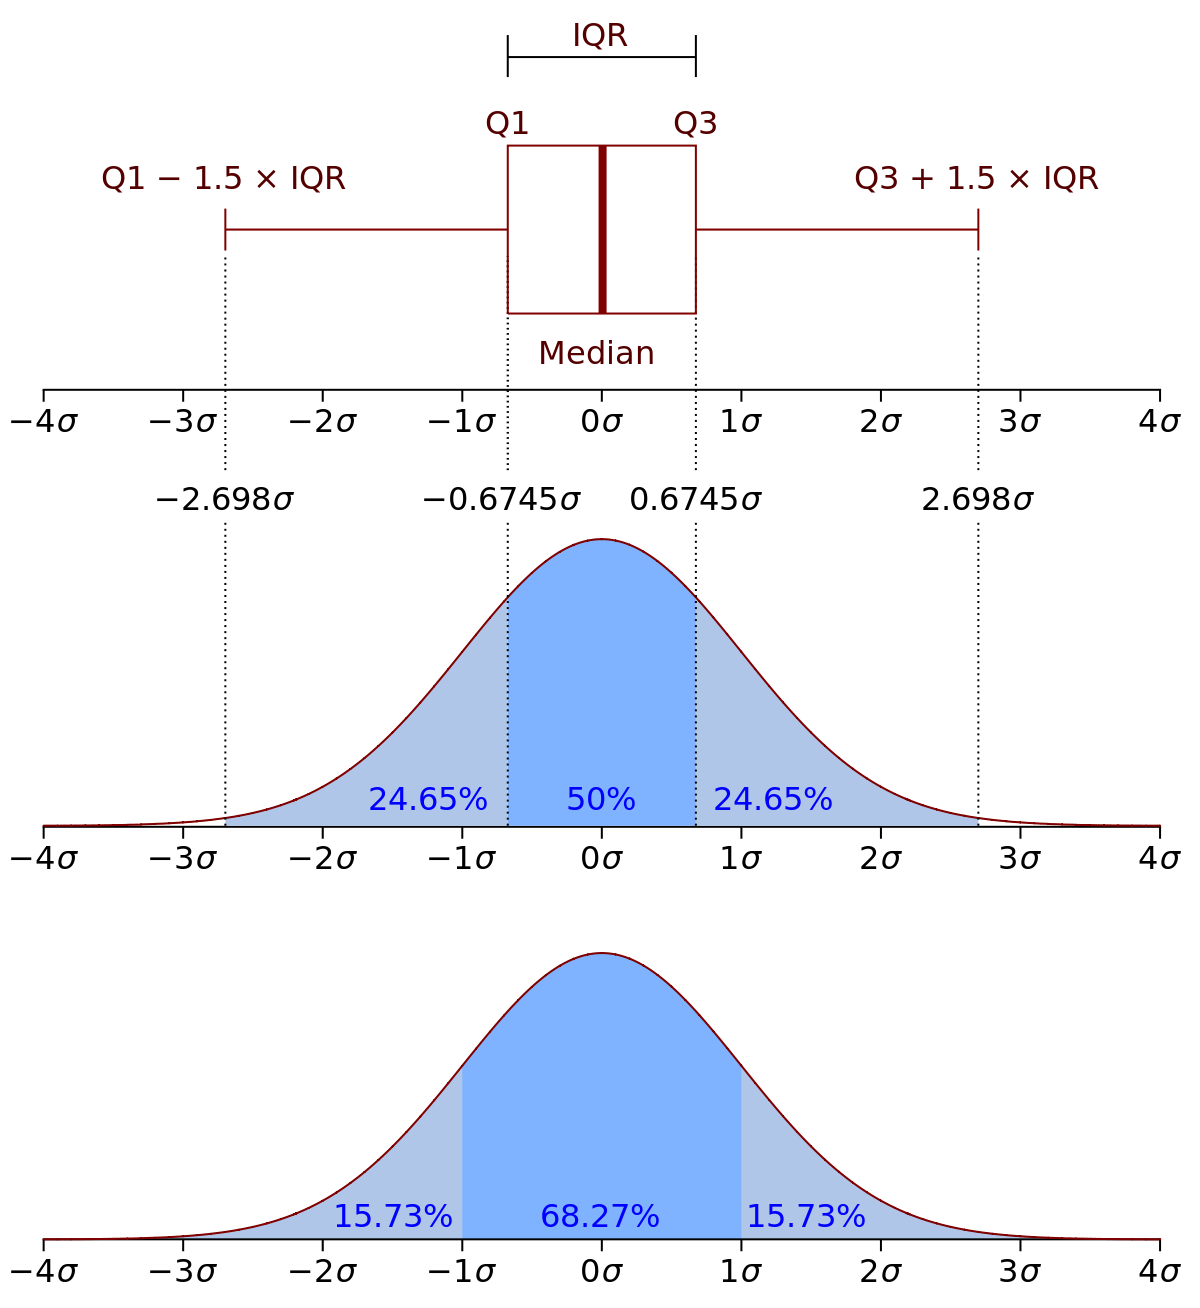
\includegraphics[scale=0.2]{TemplateTesi/immagini/iqr.png}
    \caption{IQR per rilevazione e cancellazione outlier \cite{ImmIQR}}
    \label{fig:my_label}
\end{figure}

.
\newline
L'IQR viene calcolato come:

$$IQR=Q3-Q1$$
con:
\begin{itemize}
    \item Q1= Lower Quartile 
    \item Q3= Upper Quartile
\end{itemize}





\subsection{Adattamento del Modello}

Il ML si basa sull'idea che i modelli possano apprendere dai dati e adattarsi per fare previsioni o prendere decisioni. Questo significa che il modello è rappresentato da una funzione matematica che mappa gli input ai corrispondenti output desiderati. Durante la fase di training, il modello cerca di approssimare questa funzione utilizzando un insieme di dati di addestramento.

Tuttavia, i modelli di ML possono incontrare sfide nel raggiungere un adattamento ottimale ai dati. Queste sfide possono derivare da diversi fattori, come la mancanza di rappresentatività dei dati di addestramento o la complessità del problema affrontato.


Subentrano quindi due problematiche molto frequenti ovvero:
\begin{itemize}
    \item \textbf{Overfitting}: Il modello di ML si adatta troppo ai dati di addestramento, non generalizzando bene sui nuovi dati
    \item \textbf{Underfitting}: Il modello non è in grado di adattarsi correttamente ai dati di addestramento e manca di capacità predittiva
\end{itemize}  

\begin{figure}[H]
    \centering
    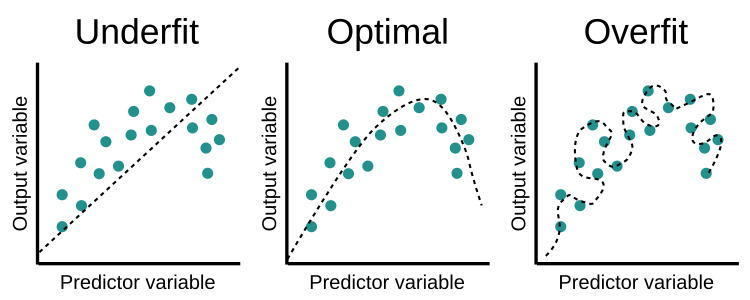
\includegraphics[scale=0.5]{TemplateTesi/immagini/fitting.png}
    \caption{Overfitting,Underfitting e fitting ottimale comparati \cite{ImmFittingComparazione}}
    \label{fig:fitting}
\end{figure}
Per affrontare questi due problemi possiamo utilizzare tecniche come la cross validation e la data augmentation:

\subsubsection{Cross Validation}
 È una tecnica ampiamente utilizzata per valutare le prestazioni di un modello di ML e affrontare il problema dell'overfitting. 
 
La cross validation (figura \ref{fig:crossvalidation}) suddivide l'insieme di dati di addestramento in K sottoinsiemi, noti come fold. Successivamente, il modello viene addestrato K volte, ogni volta utilizzando K-1 fold come dati di addestramento e il fold rimanente come dati di validazione. Questo processo di addestramento e validazione viene ripetuto K volte, in modo che ogni fold venga utilizzato almeno una volta come dati di validazione.

\begin{figure}[H]
    \centering
    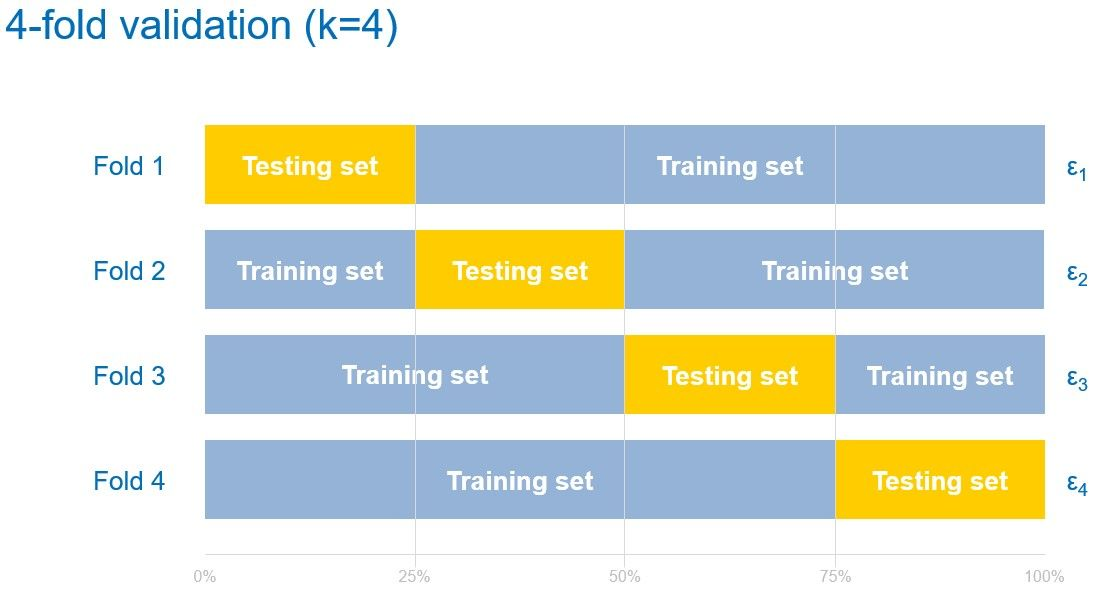
\includegraphics[scale=0.3]{TemplateTesi/immagini/kfold.jpg}
    \caption{Funzionamento della Cross Validation \cite{ImmKFOld}}
    \label{fig:crossvalidation}
\end{figure}
\subsubsection{Data Augmentation}
 Il training dei modelli può richiedere una grande quantità di dati di addestramento. 
 Tuttavia, in molte applicazioni, può essere difficile raccogliere o etichettare un numero sufficiente di dati. 
 La data augmentation è una tecnica ampiamente utilizzata per affrontare questa sfida.
 Lo scopo principale della data augmentation è aumentare la quantità e la varietà dei dati di training disponibili, al fine di migliorare le prestazioni del modello.

 Tra le tecniche principali di data augmentation troviamo ad esempio:
 \begin{itemize}
     \item Noise injection: Aggiunta di un rumore gaussiano o randomico ai dati 
     \item Generative adversarial networks (GANs): Vengono usate per generare nuovi punti o nuove immagini 
     \item Trasformazioni geometriche: utilizzate per modificare la posizione e la forma dei dati nei dataframe di immagini. Queste trasformazioni includono la traslazione, la rotazione, lo scaling, la riflessione e lo zoom (figura \ref{fig:trasformazioni})
 \end{itemize}
 

\begin{figure}[H]
    \centering
    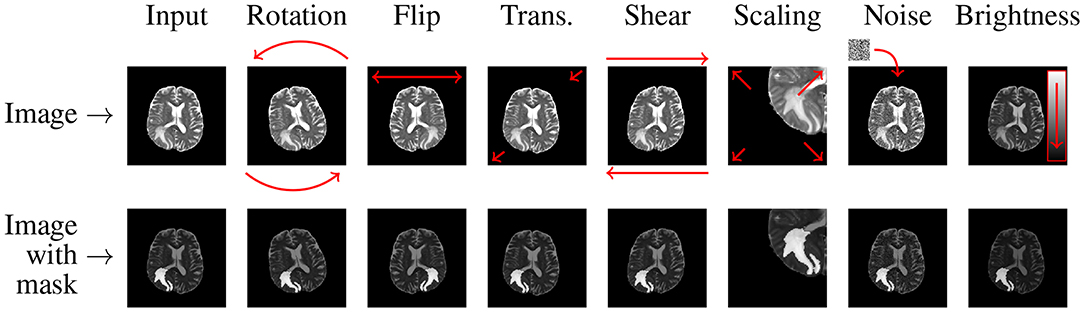
\includegraphics[scale=0.45]{TemplateTesi/immagini/fncom-13-00083-g003.jpg}
    \caption{Esempio di Data Augmentation con trasformazioni geometriche in Healthcare \cite{imm_dataaug}}
    \label{fig:trasformazioni}
\end{figure}

\subsection{Bias}
Nel contesto del ML, il termine "bias" si riferisce a una serie di problematiche che possono influenzare negativamente i modelli e le decisioni prese da essi. 
Il bias può derivare da molteplici fonti, come i dati di addestramento sbilanciati, i pregiudizi umani incorporati nei dati o negli algoritmi, o le limitazioni dei modelli stessi.
Tra le varie tipologie di bias troviamo\cite{biasgoogle}:
\begin{itemize}
    \item Reporting Bias:  si verificano quando la frequenza di eventi, o esiti catturati in un dataset non riflette accuratamente la loro frequenza nel mondo reale.
    \item Automation Bias: tendenza a favorire i risultati generati da sistemi automatizzati rispetto a quelli generati da sistemi non automatizzati,come l'ispezione da parte di un lavoratore, indipendentemente dai tassi di errore di ciascuna delle parti.
    \item Implicit Bias: si verificano quando si fanno ipotesi basate sui propri preconcetti e sulle proprie esperienze personali che non si applicano necessariamente al mondo reale.
    \begin{itemize}
        \item Confirmation Bias: Bias dove chi costruisce il modello elabora inconsciamente i dati in modo da affermare convinzioni e ipotesi preesistenti
        \item Experimenter's Bias: Bias per cui chi addestra il modello continua fino a quando non produce un risultato che si allinea con la sua ipotesi iniziale 
    \end{itemize}
\end{itemize}

L'Explainable AI accennata nel capitolo precedente( che verrà ulteriormente trattata in questo capitolo) è una valida soluzione per mitigare o comprendere i bias presenti nel nostro modello.  

\section{Metriche di Valutazione}


Nel contesto dell'analisi delle prestazioni dei modelli di ML per la classificazione binaria, è di fondamentale importanza avere una chiara comprensione dei concetti di true positive (TP), true negative (TN), false positive (FP) e false negative (FN). Questi concetti 
offrono una panoramica delle capacità predittive di un modello.

\begin{itemize}
    \item \textbf{True Positive}: si verifica quando il modello classifica correttamente un'istanza come positiva, corrispondente alla sua reale etichetta positiva.
    \item \textbf{True Negative}: il modello classifica correttamente un'istanza come negativa, in accordo con la sua reale etichetta negativa. Rappresenta il caso in cui il modello riconosce correttamente l'assenza di una condizione positiva

\item \textbf{False Positive}:  il modello classifica erroneamente un'istanza come positiva, nonostante la sua reale etichetta sia negativa. Indica un falso allarme, in cui il modello indica erroneamente la presenza di una condizione positiva quando non è effettivamente presente. 

\item \textbf{False Negative}: il modello classifica erroneamente un'istanza come negativa, nonostante la sua reale etichetta sia positiva. Questo rappresenta un errore di mancata identificazione di una condizione positiva
\end{itemize}
Ad esempio:
\begin{itemize}
    \item True Positive: nella diagnosi di una malattia, un true positive si verifica quando il modello identifica correttamente un paziente come affetto dalla malattia e il paziente  ne è effettivamente affetto. 
    \item True Negative: nella classificazione di email come spam o non spam, un true negative si verifica quando il modello correttamente identifica un'email come non spam e l'email effettivamente non è spam.
    \item False Positive:  nella diagnosi di una malattia, un false positive si verifica quando il modello indica erroneamente che un paziente è affetto dalla malattia, ma il paziente non ne è affetto
    \item False Negative: nella classificazione di email , come prima, un false negative si verifica quando il modello non riesce a riconoscere un'email come spam, nonostante l'email sia effettivamente spam
\end{itemize}


\subsection{Confusion Matrix}
La Confusion Matrix è uno strumento statistico  utilizzato per valutare le prestazioni dei modelli di classificazione.
È una matrice quadrata che visualizza il numero di campioni di dati classificati correttamente e erroneamente dal modello, in base ai valori delle metriche sopra descritte.
La confusion matrix ci permette di avere una rapida visione della classificazione dei valori, la sua struttura è rappresentata in figura \ref{fig:confusionmatrix}

\begin{figure}[H]
    \centering
    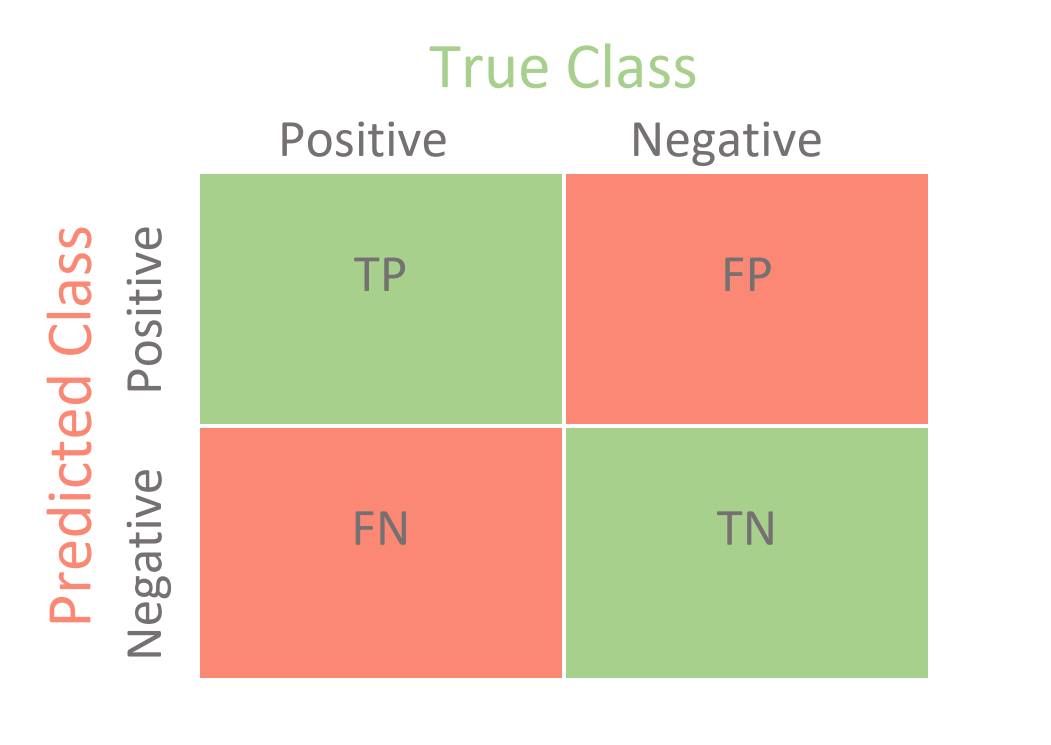
\includegraphics[width=0.5\linewidth]{TemplateTesi//immagini/confusionmatrix.png}
    \caption{Struttura della Confusion Matrix \cite{ImmConfusionMatrix}}
    \label{fig:confusionmatrix}
\end{figure}
\subsection{Accuracy, Precision e Recall}

Le metriche di valutazione nel ML, come accuracy, precision e recall, sono direttamente correlate ai concetti di true positive, true negative, false positive e false negative. Questi concetti vengono utilizzati per calcolare queste metriche e fornire una valutazione più completa delle prestazioni del modello.

Le metriche fondamentali su cui si basano anche quelle più complesse sono quindi le 3 elencate precedentemente:

\begin{itemize}
    \item \textbf{Accuracy}: Metrica che viene utilizzata per tenere traccia delle previsioni effettuate correttamente.
    Rappresenta la proporzione di campioni correttamente valutati sul totale dei campioni:
    \[\frac{Predizioni Corrette}{Predizioni Totali}\]
    o più formalmente:
    \[\frac{TP+TN}{TP+TN+FP+FN}\]
    (Non tiene traccia dei falsi negativi)
    
    \item \textbf{Recall}: Metrica che risponde alla domanda "Quale proporzione di 'Positive' è stata identificata correttamente?"
    calcolata come:

    \[\frac{TP}{TP+FN}\]
    (Non tiene traccia dei falsi positivi)


    \item \textbf{Precision}: La precision misura la percentuale di istanze positive identificate correttamente rispetto a tutte le istanze identificate come positive dal modello. In altre parole, indica quanto sia preciso il modello nel predire correttamente le istanze positive. 
    La formula per calcolare la precision è la seguente:
    \[\frac{TP}{TP+FP}\]

\end{itemize}

\section{Preprocessing}
Il preprocessing dei dati svolge un ruolo fondamentale nel ML, in questa fase risiede la preparazione dei dati per il training.
Consiste in una serie di trasformazioni e operazioni volte a rendere i dati idonei per l'apprendimento del modello. 
Nel settore dell'healthcare, il preprocessing dei dati è particolarmente cruciale, poiché i dati sanitari possono essere complessi, eterogenei e soprattutto sensibili.
Di seguito 3 procedure tipiche del preprocessing dei dati: 
\begin{itemize}
    \item \textbf{Pulizia Dati}: i dati, come anticipato, sono spesso complessi ed eterogenei.
    Possono provenire da diverse fonti, come dispositivi medici o registri elettronici. 
    Questa eterogeneità può portare a dati sporchi o incompleti, che possono influenzare negativamente l'addestramento dei modelli di ML. Pertanto, è fondamentale condurre un'attenta pulizia dei dati prima di utilizzarli per il training del modello.
    La pulizia dei dati può includere diverse attività, come la rimozione dei valori mancanti o errati, la gestione degli outlier e la standardizzazione delle variabili. Ad esempio, potrebbe essere necessario rimuovere i record dei pazienti con dati mancanti, al fine di evitare un'analisi distorta o un addestramento del modello inaccurato.
    \item \textbf{Scaling}: lo scaling dei dati è una tecnica essenziale per garantire che le variabili abbiano un impatto comparabile sul modello di ML. Lo scaling dei dati implica la trasformazione delle variabili in modo che abbiano una scala comune, riducendo così le differenze di scala tra le variabili stesse.
    tra le varie tecniche di scaling troviamo:
    \begin{itemize}
        \item Z-Score Scaling: trasforma i dati in modo che abbiano una media zero e una deviazione standard unitaria. La formula per calcolare lo Z-Score Scaling di un dato $x$ è:

        
\[x\_scaled = \frac{(x - mean)}{std}\]


        Dove "$mean$" rappresenta la media della variabile e "$std$" rappresenta la deviazione standard della variabile.

    \item Min-Max Scaling: Un'altra tecnica comune per lo scaling dei dati è il Min-Max Scaling, che trasforma i dati in un intervallo specifico, di solito compreso tra 0 e 1. La formula per calcolare il Min-Max Scaling di un dato $x$ è:

       
\[ x\_scaled = \frac{(x - min)}{max - min}\]


    Dove "$min$" rappresenta il valore minimo della variabile e "$max$" rappresenta il valore massimo della variabile. 

    \item Robust Scaling: Questa tecnica utilizza la mediana e l'intervallo interquartile (IQR) per ridimensionare i dati. La formula per calcolare la Robust Scaling di un dato $x$ è:

  
\[  x\_scaled = \frac{(x - mediana)}{IQR}\]


    Dove "$mediana$" rappresenta la mediana della variabile e "$IQR$" rappresenta l'intervallo interquartile della variabile.
    \end{itemize}
    \item \textbf{Feature Selection}:
    La feature selection è il processo di selezione delle features più rilevanti da un insieme iniziale per addestrare i modelli di ML. L'obiettivo è eliminare le caratteristiche poco informative, riducendo così la dimensione dello spazio delle caratteristiche, quindi la complessità generale del modello e migliorandone la generalizzazione. Una selezione accurata delle features può portare a modelli più semplici, che richiedono meno dati per l'addestramento e producono risultati più stabili.
\end{itemize}
\section{Modelli}
Alla base di ogni tool di AI, oltre ai dati, troviamo il modello.
Di seguito verranno illustrati vari modelli che ho tenuto in considerazione durante il mio lavoro di tesi.

\subsection{Support Vector Machine}
Le SVM (Support Vector Machine) sono un tipo di modello di apprendimento supervisionato che possono essere utilizzate per la classificazione e la regressione.
L'obiettivo delle SVM, nel contesto della classificazione, è quello di trovare un iperpiano che separi in modo ottimale i punti di dati delle diverse classi nel miglior modo possibile, dove un iperpiano è definito come un sottospazio lineare di dimensione inferiore di uno rispetto allo spazio in cui è contenuto\cite{def_iperpiano}.
\begin{figure}[H]
    \centering
    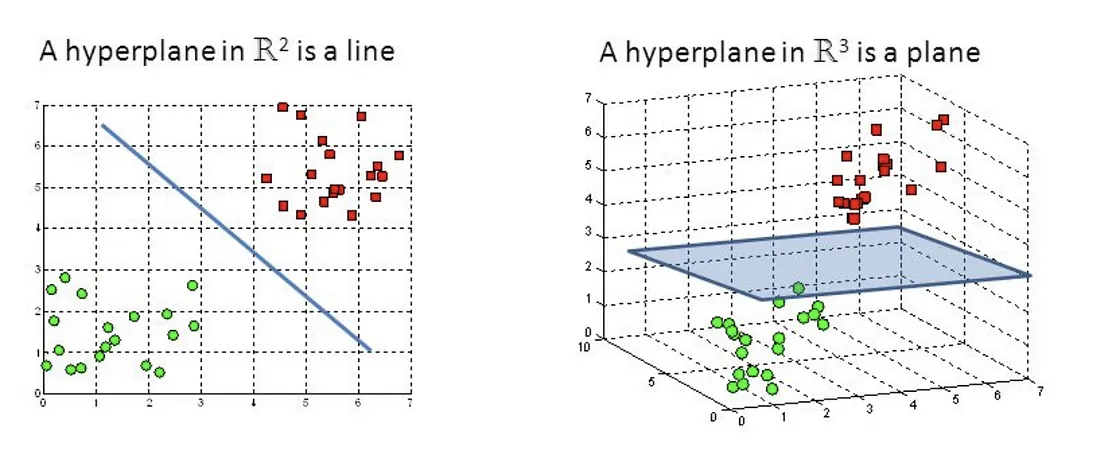
\includegraphics[width=0.7\linewidth]{TemplateTesi//immagini/1_ZpkLQf2FNfzfH4HXeMw4MQ.png}
    \caption{Esempi di Iperpiani \cite{imm_svm}}
    \label{fig:enter-label}
\end{figure}\newpage

SVM fa uso di due concetti fondamentali:

\begin{itemize}
\item \textbf{Kernel}:

     Per kernel si intende una funzione matematica che consente di mappare i dati dallo spazio delle features originale a uno spazio di dimensione superiore, dove i dati possono essere più facilmente separabili.

     L'utilizzo delle funzioni kernel è conosciuto come "kernel trick" (figura \ref{fig:kerneltrick})ed è una delle caratteristiche distintive delle SVM. La principale motivazione dietro l'utilizzo dei kernel è che, sebbene i dati nel loro spazio originale possano non essere separabili linearmente, potrebbero essere separabili in uno spazio di dimensione superiore.
    \begin{figure}[H]
        \centering
        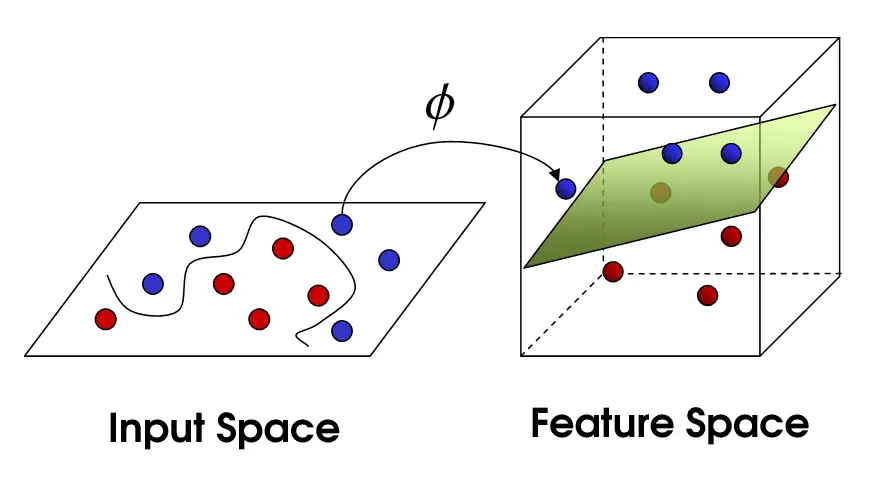
\includegraphics[width=0.6\linewidth]{TemplateTesi//immagini/1_zWzeMGyCc7KvGD9X8lwlnQ.png}
        \caption{Il Kernel Trick \cite{imm_svmkerneltrick}}
        \label{fig:kerneltrick}
    \end{figure}
    \item \textbf{Massimizzazione del Margine}:
    Il concetto di margine è fondamentale nelle Support Vector Machines e gioca un ruolo chiave nell'ottimizzazione della separazione dei dati. Il margine rappresenta la distanza tra l'iperpiano di separazione e i dati di ciascuna classe.
    L'obiettivo delle SVM quindi è quello di massimizzare il margine, poiché un margine ampio indica una migliore generalizzazione del modello e una maggiore capacità di gestire dati non visti in fase di addestramento
    \end{itemize}



\subsection{Random Forest}
Tra i modelli di ML valutati durante il mio lavoro di tesi, il Random Forest si è dimostrato il più performante. Questo modello si basa sull'utilizzo degli alberi decisionali e sfrutta il concetto di entropia per creare una foresta di alberi decisionali, con i quali effettuare le predizioni.

\subsubsection{Entropia di Shannon}
L'entropia può essere definita come una misura che quantifica il livello di disordine o incertezza presente in un sistema.
Nel contesto del ML, si traduce in un concetto derivato dalla teoria dell'informazione di Claude Shannon. Rappresenta quindi la quantità di informazione media contenuta in un insieme di dati. Maggiore è l'entropia, maggiore è l'incertezza o il disordine nell'insieme di dati.

L'entropia di un insieme $S$ con $n$ possibili classi $i$ , denotate come \(\{i_1, i_2, ..., i_n\}\), può essere quindi calcolata utilizzando la seguente formula:
$$E(S) = -\sum_{i=1}^{n} (p_i \log_2(p_i))$$

Nel contesto di utilizzo di un modello di ML il nostro obiettivo è quello di minimizzare l'entropia dei gruppi generati dal modello.

\subsubsection{Alberi Decisionali}
\begin{figure}[H]
    \centering
    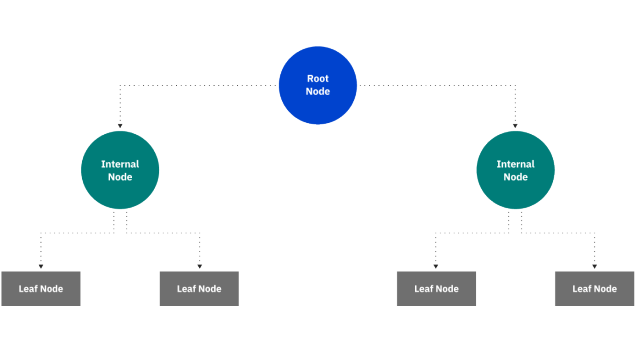
\includegraphics[width=0.7\linewidth]{TemplateTesi/immagini/alberodecibmstruttura.png}
    \caption{Struttura di un albero decisionale \cite{ibmdecisiontrees}}
    \label{fig:ibmtrees_struttura}
\end{figure}
Un albero decisionale è un algoritmo di apprendimento supervisionato, utilizzato sia per attività di classificazione che di regressione \cite{ibmdecisiontrees}. Si compone di una struttura ad albero gerarchica, che consiste di un nodo radice, di rami, nodi interni e nodi foglia (figura \ref{fig:ibmtrees_struttura}) , ogni nodo rappresenta un test su una feature e ogni ramo rappresenta il risultato di quel test, come vediamo in figura \ref{fig:ibmtrees}.

Gli alberi decisionali sono costruiti utilizzando algoritmi che cercano di dividere l'insieme di dati in sottoinsiemi omogenei. La divisione viene effettuata in modo iterativo selezionando le caratteristiche e i test che massimizzano la riduzione dell'incertezza e quindi quello che viene chiamato "Information Gain"(IG), selezionando la suddivisione che produce meno entropia nei dati.

$$IG = E(parent) - E(child)$$

\begin{figure}[H]
    \centering
    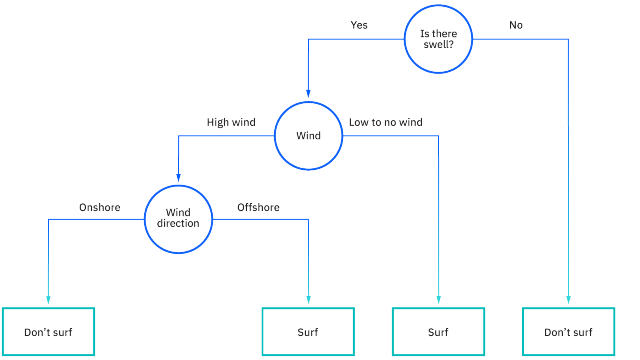
\includegraphics[width=0.7\linewidth]{TemplateTesi//immagini/alberidecisionaliibm.png}
    \caption{Funzionamento Albero Decisionale \cite{ibmdecisiontrees}}
    \label{fig:ibmtrees}
\end{figure}

\subsubsection{Creazione della Foresta}
La foresta di alberi decisionali che compongono il concetto di "Random Forest" viene creata seguendo il concetto di "ensemble learning",una tecnica che combina diversi modelli di apprendimento per ottenere prestazioni migliori rispetto al singolo modello. Nel
caso del random forest, l'ensemble è costituito da un insieme di alberi decisionali.

Per creare ciascun albero decisionale, viene utilizzato un sottoinsieme casuale dei dati di addestramento. Questa tecnica viene chiamata "bagging" (figura \ref{fig:bagging}).
Si compone partendo da due concetti chiave: il bootstrap e l'aggregazione.
\begin{figure}[H]
    \centering
    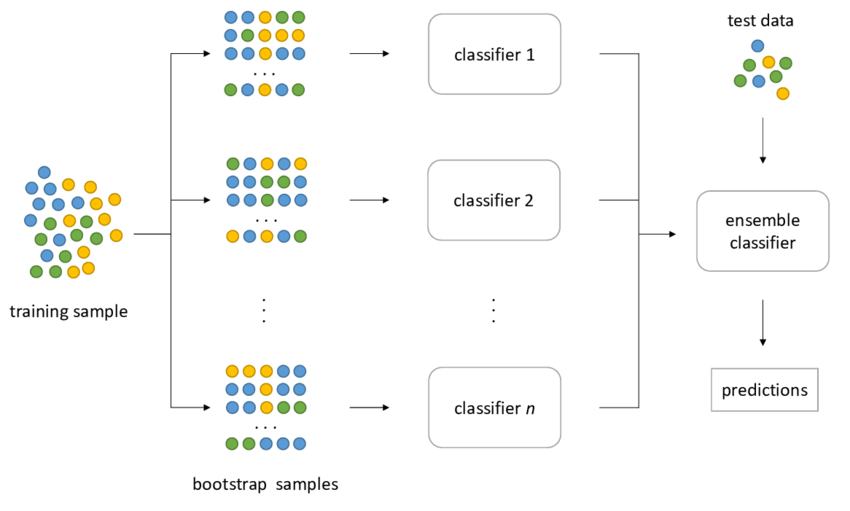
\includegraphics[width=0.8\linewidth]{TemplateTesi//immagini/bagging-1.png}
    \caption{Tecnica "Bagging" \cite{immbagging}}
    \label{fig:bagging}
\end{figure}

\begin{itemize}
    \item \textbf{Il Bootstrap} è un metodo di campionamento che prevede la selezione casuale di campioni dall'insieme di dati di training, consentendo la possibilità che un campione venga selezionato più volte o non venga selezionato affatto. Questo processo di selezione ci permette di creare diversi sottoinsiemi di dati a partire dal nostro insieme di addestramento.

    \item \textbf{L'aggregazione} viene effettuata combinando le previsioni dei singoli modelli creati utilizzando i sottoinsiemi di dati generati tramite il bootstrap. Nel caso del random forest, le previsioni dei singoli alberi decisionali vengono combinate per dare in output il risultato della foresta di alberi decisionali (figura \ref{fig:randomforest})
\end{itemize}
\begin{figure}[H]
    \centering
    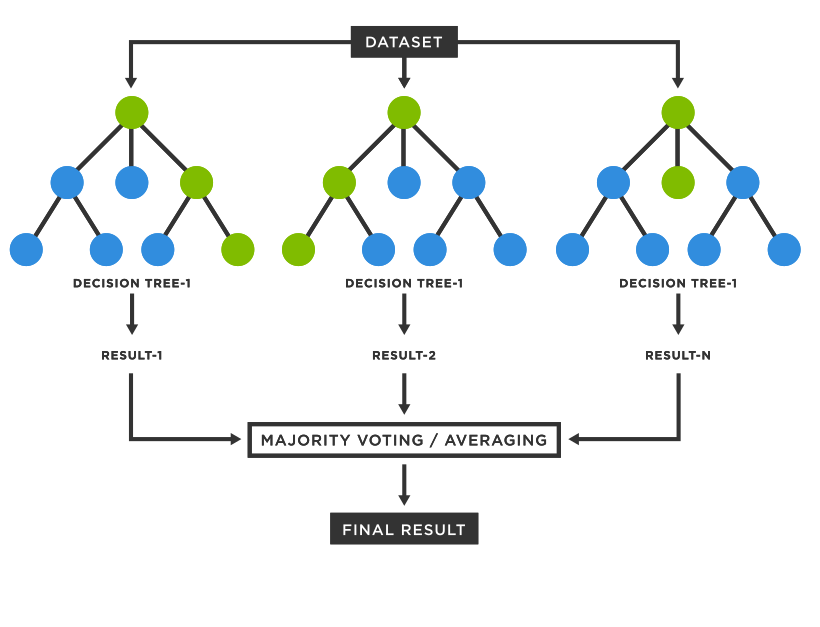
\includegraphics[width=0.7\linewidth]{TemplateTesi//immagini/random-forest-diagram.png}
    \caption{Processo decisionale all'interno del Random Forest \cite{immrf}}
    \label{fig:randomforest}
\end{figure}
\subsection{eXtreme Gradient Boosting}
Extreme Gradient Boosting (XGB)\cite{XGB} è un algoritmo di ML che, come random forest, si basa sul concetto di ensemble, ovvero sfrutta una aggregazione di modelli di conoscenza più deboli per ottenere una predizione più accurata; ogni nuovo albero viene addestrato sugli errori del precedente in un processo detto boosting.

Il termine "gradient boosting" deriva dall'idea di "potenziare" o migliorare un singolo modello "debole" combinandolo con una serie di altri modelli deboli per generare un modello "forte" collettivo. Il gradient boosting è un'estensione del boosting in cui il processo di generazione dei modelli deboli è formalizzato come un algoritmo "gradient descent" su una funzione obiettivo.
Il Gradient Boosting genera risultati mirati per il modello successivo nel tentativo di minimizzare gli errori.
Le loss function utilizzabili con XGB variano in base al contesto di utilizzo, nel caso della classificazione binaria è generalmente utilizzata la "Log Loss", questa quantifica il prezzo pagato per l'imprecisione delle previsioni nei problemi di classificazione. La log loss penalizza gli errori nella classificazione tenendo conto della probabilità di classificazione \cite{xgbloss1,xgbloss2,XGBNvidia}. 

\subsection{Adaptive Boosting }
Adaptive Boosting (ADA) rappresenta un algoritmo di boosting che mira a creare un classificatore forte combinando una serie di classificatori deboli. Questi classificatori deboli, noti come "decision stump" ( alberi decisionali con una sola diramazione), vengono utilizzati come punto di partenza per la costruzione graduale del modello finale. 
Durante il processo, vengono assegnati pesi equi a ogni record classificato e successivamente si attribuiscono pesi più significativi alle classificazioni errate, in modo da creare un nuovo modello debole\cite{ada1}. Questi passaggi vengono ripetuti fino a quando i modelli deboli generati, ognuno con pesi diversi, vengono aggregati in un unico modello forte in grado di eseguire la classificazione in maniera efficace, come visibile in figura \ref{fig:ada}\cite{ada2}.

\begin{figure}[H]
    \centering
    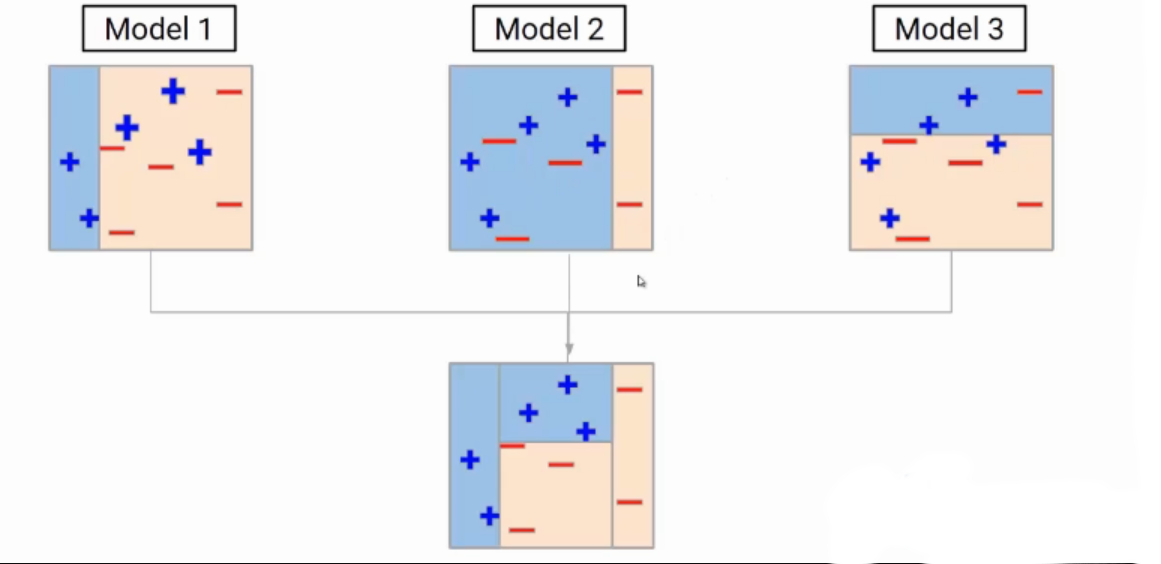
\includegraphics[width=0.75\linewidth]{TemplateTesi//immagini/dsd.jpg}
    \caption{Processo di creazione del modello forte per ADA \cite{ada2}}
    \label{fig:ada}
\end{figure}
\section{Tuning degli iperparametri}
Nel ML, gli iperparametri sono parametri esterni al modello che ne descrivono le caratteristiche. Attraverso il processo di "tuning degli iperparametri", si ricerca la combinazione ottimale di valori per questi parametri al fine di massimizzare le prestazioni del modello. L'obiettivo è trovare i valori migliori per gli iperparametri che permettano di ottenere il miglior modello possibile.

Due tecniche utilizzate per la ricerca degli iperparametri sono:
\begin{itemize}
    \item \textbf{Random Search}:
    un metodo di tuning degli iperparametri che coinvolge la selezione casuale dei valori degli stessi all'interno di un certo intervallo. Durante il processo di Random Search, vengono generate diverse combinazioni casuali di valori degli iperparametri e viene addestrato un modello per ciascuna combinazione. Successivamente, le prestazioni di ogni modello vengono valutate utilizzando una metrica di valutazione appropriata, come l'accuracy. Infine, si seleziona la combinazione di iperparametri che ha fornito le migliori prestazioni
    \item \textbf{Grid Search}:
    La Grid Search prevede la definizione di una griglia di possibili valori per ciascun iperparametro. Per ogni combinazione di valori degli iperparametri nella griglia, viene addestrato un modello e le sue prestazioni vengono valutate utilizzando le metriche di valutazione scelte.

    Il processo di Grid Search esplora in maniera sistematica tutte le possibili combinazioni di valori degli iperparametri specificate nella griglia. Ad esempio, se abbiamo due iperparametri A e B con tre possibili valori per A e due possibili valori per B, la Grid Search esplorerà un totale di sei combinazioni.
\end{itemize}
Spesso tali tecniche sono usate in combinazione con processi di cross validation, spiegati precedentemente
\section{PostProcessing: XAI}
L'opacità e la mancanza di trasparenza dei  modelli di ML possono portare a dubbi sulla loro affidabilità e accettabilità. L'Explainable Artificial Intelligence (XAI) è emersa come una disciplina che mira a risolvere questo problema, cercando di rendere i modelli di ML più comprensibili e interpretabili per gli esseri umani.

L'obiettivo fondamentale della XAI è quello di fornire spiegazioni comprensibili sul perché un modello di ML ha preso una determinata decisione o ha fatto una determinata previsione. Queste spiegazioni possono aiutare gli utenti a comprendere il ragionamento del modello e a identificare potenziali pregiudizi, errori o vulnerabilità nel processo decisionale. La trasparenza e l'interpretabilità dei modelli di IA sono diventate sempre più importanti in diversi contesti, come la medicina, la finanza, la sicurezza e molti altri settori in cui le decisioni basate sull'IA possono avere conseguenze significative sulla vita delle persone \cite{aicambiatutto}.


La XAI comprende due approcci principali: \textbf{model-based} e \textbf{post-hoc}.
L'approccio model-based si concentra sulla costruzione di modelli interpretabili fin dall'inizio. Questi modelli sono progettati per essere esplicitamente interpretabili e trasparenti, consentendo agli utenti di comprendere facilmente le decisioni prese.

D'altra parte, l'approccio post-hoc si concentra sulla spiegazione dei modelli di ML "black box" , che possono essere complessi e difficili da interpretare. L'obiettivo è fornire spiegazioni esterne al modello stesso, senza modificarne la struttura. Questo approccio è particolarmente utile quando si lavora con modelli di ML complessi come le Deep Neural Network (DNN). Alcuni esempi di approcci post-hoc includono LIME (Local Interpretable Model-Agnostic Explanations) e SHAP (SHapley Additive exPlanations), che generano spiegazioni locali per le singole previsioni.

Oltre alla distinzione tra approcci model-based e post-hoc, è possibile classificare i modelli di ML in \textbf{white box} e \textbf{black box}. I modelli white box sono quelli in cui la struttura e il funzionamento sono completamente trasparenti e comprensibili. Esempi di modello white box sono la linear regression, in cui i coefficienti delle variabili di input forniscono informazioni dirette sul loro impatto sul risultato, e il decision tree dove la struttura dell'albero ci fornisce i dettagli sul processo decisionale (come visibile in figura \ref{fig:ibmtrees}). Al contrario, i modelli black box sono caratterizzati da una mancanza di trasparenza e comprensibilità.Le DNN sono un esempio di modello black box, poiché la complessità delle loro connessioni rende difficile comprenderne il funzionamento.

Nel contesto della XAI, sono anche rilevanti i concetti di \emph{agnosticismo} e di \emph{scope}. Le spiegazioni, frutto della XAI, possono essere categorizzate come \textbf{model-agnostic} o \textbf{model-specific} e, dal punto di vista dello scope,  \textbf{global explanation} o \textbf{local explanation}.

Le spiegazioni model-agnostic sono indipendenti dal modello di ML utilizzato e sono applicabili a una vasta gamma di modelli. Queste spiegazioni cercano di estrarre informazioni  rilevanti per la comprensione generale del modello. Ad esempio, SHAP è un approccio model agnostic che calcola l'importanza delle caratteristiche per una specifica previsione.

D'altra parte, le spiegazioni model-specific sono specifiche per un determinato modello di ML. Queste spiegazioni sfruttano le proprietà interne del modello per fornire spiegazioni dettagliate delle decisioni prese. Ad esempio, le attribuzioni dei pesi delle connessioni neurali in una GAN sono spiegazioni specifiche che evidenziano il contributo di ogni connessione alla generazione dei dati.

Le spiegazioni globali sono orientate a fornire una comprensione generale del modello di ML nel suo complesso. Queste spiegazioni esaminano le regole generali e le relazioni tra le variabili di input e output. Le spiegazioni locali, invece, si concentrano su singole istanze o previsioni, offrendo una comprensione dettagliata dei fattori che hanno contribuito a una specifica decisione.


\subsection{LIME}
LIME, abbreviazione di Local Interpretable Model-Agnostic Explanations, è una tecnica appartenente all'Explainable Artificial Intelligence (XAI). Essa si basa sull'utilizzo di "Modelli Locali Surrogati" per spiegare le decisioni prese dal modello di ML in esame. Il funzionamento di LIME si basa sull'addestramento di tali modelli surrogati.

Per comprendere le motivazioni alla base di una specifica previsione, LIME esegue una serie di test sulle previsioni quando vengono variati i valori delle features nei dati del modello generale. A tal fine, LIME genera un nuovo insieme di dati costituito da campioni perturbati e le relative previsioni del modello generale. Successivamente, su questo nuovo insieme di dati, LIME addestra un modello surrogato locale, che viene pesato in base alla vicinanza delle istanze campionate rispetto all'istanza di interesse iniziale. L'obiettivo del modello surrogato ottenuto è quello di essere una buona approssimazione delle previsioni del modello di ML a livello locale, senza necessariamente essere un'ottima approssimazione globale. Questo tipo di precisione è definito anche come fedeltà locale.\cite{interpretableml}

Dal punto di vista matematico il funzionamento del modello surrogato è descritto nella seguente maniera 

$$\text{explanation}(x)=\arg\min_{g\in{}G}L(f,g,\pi_x)+\Omega(g)$$

dove:
\begin{itemize}
   \item x= Dato in input (un record)
    \item f= Modello generale
    \item g= Modello surrogato
    \item G= Famiglia di modelli interpretabili
    \item \(\pi_x\)= misura di prossimita ad x
    \item \(\Omega(g)\)= usato per regolare la complessità del modello surrogato g
    \item \(L(f,g,\pi_x)\)= misurerà l'infedeltà di g nel fare approssimazioni di f nella località $\pi_x$.
\end{itemize}
ottenendo così i seguenti passaggi fondamentali:
\begin{itemize}
    \item Si seleziona l'istanza per la quale si desidera avere una spiegazione della previsione del modello black box.
    \item Si perturba il dataset e si calcolano le previsioni del modello black box per il nuovo dataset pesando i nuovi dati in base alla loro vicinanza con l'istanza scelta.
    \item Si addestra il modello surrogato sul set di dati con le variazioni.
    \item Otteniamo la previsione della istanza iniziale interpretando il modello locale surrogato.
\end{itemize}
\begin{figure}[H]
    \centering
    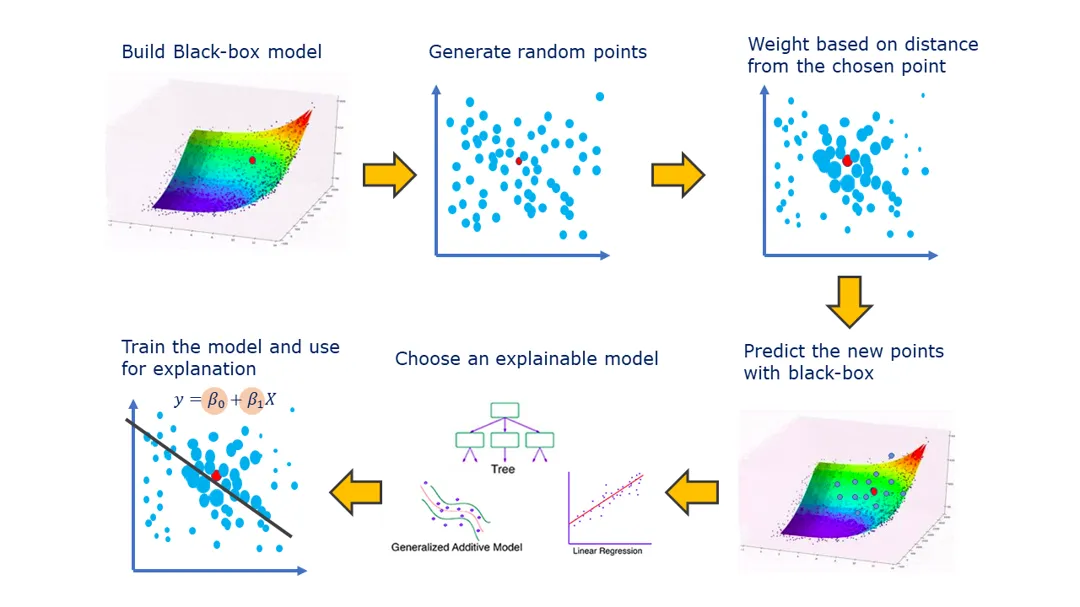
\includegraphics[width=1\linewidth]{TemplateTesi//immagini/limesteps.png}
    \caption{Steps di LIME \cite{immstepslime}}
    \label{fig:enter-label}
\end{figure}
\subsection{SHAP}
SHAP, acronimo di SHapley Additive exPlanations, è una tecnica di XAI che trova le sue radici nella teoria dei giochi. In particolare, si basa sul concetto di Shapley Values.
Nella teoria dei giochi, gli Shapley Values sono una misura del contributo che ciascun giocatore apporta in un gioco cooperativo. Nel contesto della teoria dei giochi, consideriamo una "coalizione" come un gruppo di persone diverse che collaborano durante lo svolgimento di un gioco. Gli Shapley Values ci forniscono una misura di quanto ciascun giocatore abbia contribuito all'interno della coalizione.
In modo più formale, il valore di Shapley del valore \emph{val} di una feature è il suo contributo al risultato finale, ponderato e sommato su tutte le possibili combinazioni di valori delle features. Questo concetto può essere espresso mediante la seguente formula \cite{interpretableml}:
$$\phi_j(val)=\sum_{S\subseteq\{1,\ldots,p\} \backslash \{j\}}\frac{|S|!\left(p-|S|-1\right)!}{p!}\left(val\left(S\cup\{j\}\right)-val(S)\right)$$
dove  $S$ è un sottoinsieme delle features utilizzate nel modello e $p$ il numero di caratteristiche.  

Definito $x$ come il vettore dei valori delle features dell'istanza da spiegare,
\(val_x(S)\) è la previsione per i valori delle features nell'insieme S che sono marginalizzati rispetto alle caratteristiche non incluse nell'insieme S:
$$val_{x}(S)=\int\hat{f}(x_{1},\ldots,x_{p})d\mathbb{P}_{x\notin{}S}-E_X(\hat{f}(X))$$

Il funzionamento di SHAP quindi consiste nel calcolo degli Shapley Values per ogni feature e istanza in input, offrendo in output una spiegazione su come ciascuna feature contribuisce alla previsione del modello.
Come visibile in figura \ref{fig:risultatiSHAP}
per ogni feature presente nel grafo è riportato il valore del proprio shapley value,andando a darci una rappresentazione dell'apporto di ogni feature per la risoluzione del problema in analisi.
In questo caso ci vengono presentati in ordine decrescente di impatto sulla classificazione, mostrandoci come le features "MedInc" e "Latitude" abbiano contribuito in modo positivo nella scelta di una delle due classi del problema, la feature "Longitude", invece, ha contribuito nel senso opposto alle prime due.
\begin{figure}[H]
    \centering
    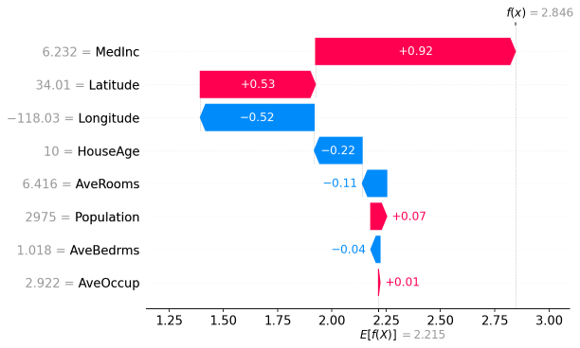
\includegraphics[width=0.75\linewidth]{TemplateTesi//immagini/shapexample.png}
    \caption{Esempio di Visualizzazione risultati di SHAP \cite{ImmShapExample}}
    \label{fig:risultatiSHAP}
\end{figure}


\subsection{Counterfactual Explanations}
Counterfactual Explanations è una tecnica che fornisce una  spiegazione sui risultati di un modello che si basa sulla modifica dei valori delle features di un'istanza in input al fine di comprendere come tali modifiche influenzino le decisioni dello stesso.
In particolar modo una "counterfactual explanation" di una predizione ci \textbf{descrive i cambiamenti più piccoli da effettuare sui valori delle features affinchè la predizione fornita dal modello cambi} (figura \ref{fig:counterfactual}).
Ritengo importante sottolineare l'importanza dell'utilizzo di questa tecnica nel contesto della riabilitazione, poiché non solo è essenziale adottare le tecniche specifiche indicate dai professionisti, ma anche adattare il proprio stile di vita in base agli obiettivi desiderati,le spiegazioni generate possono essere un suggerimento sul percorso da seguire per rientrare nei propri obiettivi.


Il processo di generazione delle conterfactual explanations coinvolge diverse fasi. Inizialmente, viene selezionato un campione per cui si desidera ottenere una spiegazione. Successivamente, vengono applicate modifiche al campione in input per creare un'istanza alternativa. Queste modifiche possono riguardare una o più features, modificandone i valori e potendo selezionare sia le features da modificare che il range della possibile modifica.

Le modifiche effettuate sulle features possono avvenire seguendo meccanismi differenti \cite{interpretableml}:
\begin{itemize}
    \item Variazioni Randomiche: Si perturbano in maniera casuale le features, all'interno degli eventuali range indicati, valutandone poi l'outcome del modello.

    \item Algoritmi Genetici: 
    
    È possibile utilizzare algoritmi genetici come il Nondominated Sorting Genetic Algorithm (NSGA-II), questo prende ispirazione e applica le leggi di Darwin sulla "Survival of the fittest" o "Sopravvivenza del più adatto" dove il più adatto è la counterfactual explanation che minimizza un vettore di funzioni obiettivo $(o_1,o_2,o_3,o_4)$.
    \item Approccio di Wachter:

    
    Consiste nella minimizzazione della seguente "loss function"
    $$L(x,x^\prime,y^\prime,\lambda)=\lambda\cdot(\hat{f}(x^\prime)-y^\prime)^2+d(x,x^\prime)$$
    dove:
    \begin{itemize}
        \item Il primo termine è la distanza al quadrato tra la previsione del modello per il counterfactual x' e il risultato desiderato y'
        \item  Il secondo termine è la distanza d tra l'istanza x da spiegare e il counterfactual x'
        \item d è definita come la distanza di Manhattan pesata con l'inverso della deviazione mediana assoluta di ogni feature (MAD)
        $$d(x,x^\prime)=\sum_{j=1}^p\frac{|x_j-x^\prime_j|}{MAD_j}$$

        \item il parametro \( \lambda \)  serve per il bilanciamento dei contributi del primo e secondo termine all'interno della loss function 
    \end{itemize}
    
\end{itemize}
\begin{figure}[H]
    \centering
    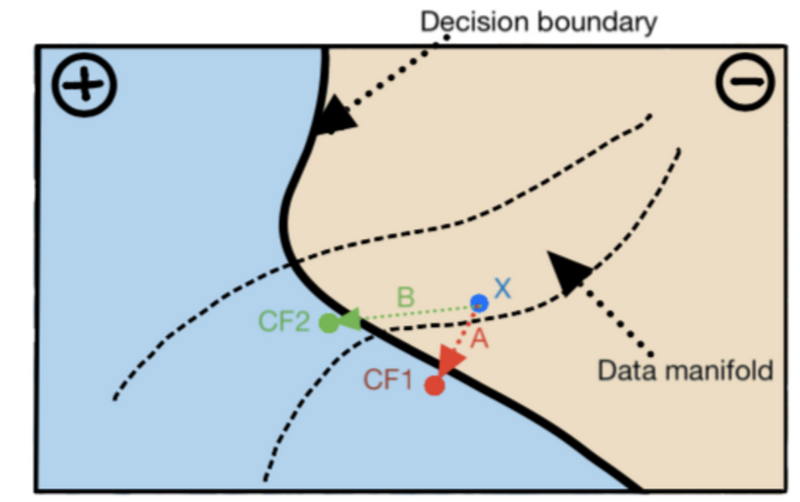
\includegraphics[width=0.7\linewidth]{TemplateTesi//immagini/cf.png}
    \caption{Funzionamento Grafico della Counterfactual Explanations \cite{immcf}}
    \label{fig:counterfactual}
\end{figure}


\section{Explorative Data Analysis (EDA)}
L'EDA svolge un ruolo cruciale nei processi di ML. Prima di poter applicare algoritmi di ML sui dati, è necessario comprendere la loro natura e struttura. 
L'EDA fornisce una panoramica iniziale che aiuta a rispondere a domande chiave come: quali variabili sono rilevanti per il problema in esame? Esistono correlazioni o pattern che possono influire sulla performance del modello? Sono presenti valori mancanti o outliers che richiedono un'attenzione particolare?
È quindi una fase fondamentale per il processo di costruzione di un modello.

Di seguito verranno elencate alcune delle tecniche o valori da tenere in considerazione durante questa fase di esplorazione dei dati.
\subsection{Distribuzione di Probabilità Normale}
In Data Science,il calcolo  della distribuzione normale è uno strumento ampiamente utilizzato per descrivere e analizzare le distribuzioni delle variabili.
La distribuzione normale, anche nota come distribuzione di Gauss, è una distribuzione continua simmetrica che rappresenta molte variabili nel mondo reale. È caratterizzata dalla sua forma a campana ( figura \ref{fig:distrnorm}) e dalla sua funzione di densità di probabilità definita dalla seguente equazione:
$$f(x,\mu, \sigma) = \frac{1}{{\sigma \sqrt{2\pi}}} \cdot e^{-\frac{{(x - \mu)^2}}{{2\sigma^2}}}$$
dove:
\begin{itemize}
    \item $\sigma^2$=varianza
    \item $\mu$=media
\end{itemize}  



\begin{figure}[H]
    \centering
    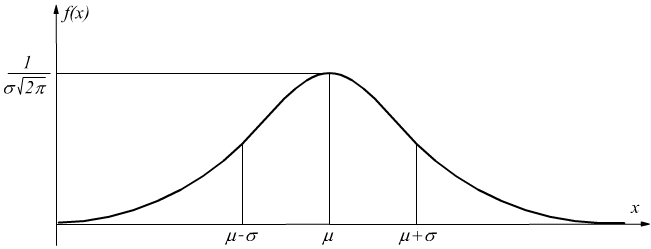
\includegraphics[width=0.5\linewidth]{TemplateTesi//immagini/distribuzionenormale.png}
    \caption{ Forma classica di una Distribuzione Normale \cite{ImmGaussiana}}
    \label{fig:distrnorm}
\end{figure}
\subsection{Coefficiente di Correlazione: HeatMap}
Il coefficiente di correlazione è una misura statistica che indica la relazione tra due variabili. Questo coefficiente varia da -1 a 1, dove un valore di -1 indica una correlazione negativa perfetta, 1 indica una correlazione positiva perfetta e 0 indica una mancanza di correlazione lineare tra le variabili.

Per calcolare il coefficiente di correlazione tra due variabili X e Y, possiamo utilizzare la seguente formula:

$$\rho(X,Y)=\frac{\sigma{_X_Y}}{\sigma_X \sigma_ Y}$$
dove:
\begin{itemize}
    \item $\sigma{_X_Y}$=covarianza tra X e Y
    \item $\sigma_X$=deviazione standard di X
    \item $\sigma_Y$=deviazione standard di Y
\end{itemize}

Uno dei metodi di visualizzazione più comodi per questa fase esplorativa è la visualizzazione tramite HeatMap dei valori dei coefficienti di correlazione tra le features, visibile in figura \ref{fig:heatmapesempio}.
\begin{figure}[H]
    \centering
    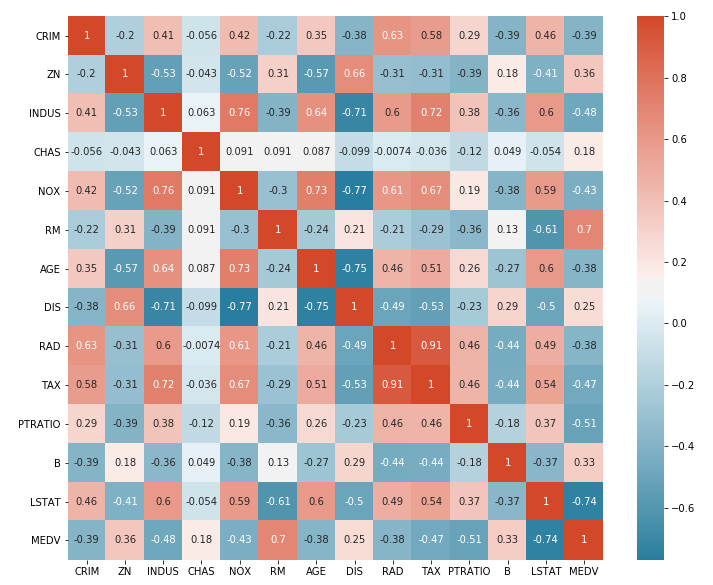
\includegraphics[width=0.5\linewidth]{TemplateTesi//immagini/heatmap esempio.png}
    \caption{Esempio di una Heatmap \cite{ImmHeatMap}}
    \label{fig:heatmapesempio}
\end{figure}
\subsection{MI (Mutual Information) Score}
Tecnica appartenente alla Teoria della Probabilità, calcola la mutua dipendenza di due variabili aleatorie, nel contesto dell'EDA è usata come tecnica di feature selection.
Viene calcolata con la seguente formula:


$$MI(X, Y) = \sum\limits_{y \in Y}\sum\limits_{x \in X} p(x, y) \log \left( \frac{p(x, y)}{p_1(x) \cdot p_2(y)} \right)
$$

dove :
\begin{itemize}
    \item p(x,y):Funzione di distribuzione di probabilità congiunta di X e Y
    \item $p_1(x)$=funzione di distribuzione di probabilità marginale di X
    \item $p_2(y)$=funzione di distribuzione di probabilità marginale di X
\end{itemize}
\end{flushleft}
